\fontfamily{\sfdefault}\selectfont
% XCircuit output "lf_quant_noise_model.tex" for LaTeX input from lf_quant_noise_model.ps
\def\putbox#1#2#3#4{\makebox[0.00000in][l]{\makebox[#1][l]{}\raisebox{\baselineskip}[0.00000in][0.00000in]{\raisebox{#2}[0.00000in][0.00000in]{\scalebox{#3}{#4}}}}}
\def\rightbox#1{\makebox[0.00000in][r]{#1}}
\def\centbox#1{\makebox[0.00000in]{#1}}
\def\topbox#1{\raisebox{-0.60\baselineskip}[0.00000in][0.00000in]{#1}}
\def\midbox#1{\raisebox{-0.20\baselineskip}[0.00000in][0.00000in]{#1}}
   \scalebox{1}{
   \normalsize
   \parbox{2.33750in}{
   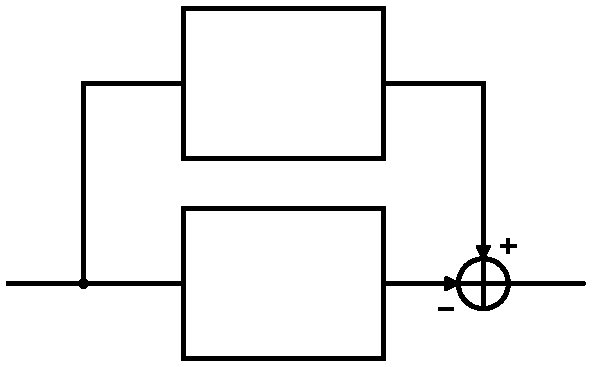
\includegraphics[scale=0.60000]{./figs/lf_quant_noise_model.pdf}\\
   % translate x=448 y=448 scale 0.38
   \putbox{0.93600in}{1.08600in}{0.96}{$\text{H}_{LF}$(z)}%
   \putbox{0.93600in}{0.43200in}{0.96}{$\hat{\text{H}}_{LF}$(z)}%
   \putbox{0.98400in}{0.28200in}{0.84}{(B-bit}%
   \putbox{0.88200in}{0.13200in}{0.84}{quantized)}%
   \putbox{0.06000in}{0.43200in}{0.96}{w[n]}%
   \putbox{2.08200in}{0.43200in}{0.96}{q[n]}%
   \putbox{1.58400in}{1.23600in}{0.96}{y[n]}%
   \putbox{1.58400in}{0.43200in}{0.96}{$\hat{\text{y}}$[n]}%
   } % close 'parbox'
   } % close 'scalebox'
   \vspace{-\baselineskip} % this is not necessary, but looks better
\fontfamily{\rmdefault}\selectfont
